\documentclass[journal=jacsat,manuscript=article]{achemso}
\usepackage[parfill]{parskip}
\usepackage[version=3]{mhchem} % Formula subscripts using \ce{}
\usepackage[section]{placeins}
\newcommand*\mycommand[1]{\texttt{\emph{#1}}}
\title{SurfinPy v2: A Phase Diagram Generator}

\author{Joshua S. Tse}
\affiliation{Department of Chemistry, University of Huddersfield, Queensgate, Huddersfield HD1 3DH, UK}
\author{Adam R. Symington}
\email{A.R.Symington@bath.ac.uk}
\affiliation{Department of Chemistry, University of Bath, Claverton Down, Bath BA2 7AY, UK}
\author{Marco Molinari}
\affiliation{Department of Chemistry, University of Huddersfield, Queensgate, Huddersfield HD1 3DH, UK}
\author{Arnaud Marmier}
\affiliation{UWE}
\author{Stephen C. Parker}
\email{S.C.Parker@bath.ac.uk}
\affiliation{Department of Chemistry, University of Bath, Claverton Down, Bath BA2 7AY, UK}

\date{2020\\ September}

\begin{document}


\textbf{Paper DOI:}  \\
\textbf{Software Repository:} https://github.com/symmy596/SurfinPy \\
\textbf{Software Archive:}  \\

\section{Summary}
SurfinPy is a python module for generating phase diagrams from DFT data.  The previous code release, reported in Adam R. Symington \textit{et. al.}\cite{Symington2019},  solved the free energy calculation  for surfaces under different constants, the most stable phase at specific temperature and pressure is then used to generate a phase diagram.  These phase diagrams can and have been used to provide an understanding of surface composition under various environmental conditions, thus providing crucial information for a range of materials science problems \cite{Symington2020a,Symington2020b,Symington2020c,Moxon2020}.

This SurfinPy release makes the following contributions (1) generic updates to the original code base to improve performance and streamline workflow, (2) introduces the new capability to calculate phase diagrams for bulk phases, and (3) allows the calculation of vibrational entropy and zero point energy for solid phases and introduce these values in to the phase diagram generation.

The largest contribution to this release is the ability to calculate and plot phase diagrams for bulk phases.  This expands the current code base to calculate the free energy for bulk phases under various pressures and temperatures.  Similarly, to the surface module free energies for each phase are calculated under a specific temperature and pressure which is then used to generate phase diagrams for bulk phases.  Temperature ranges can now be provided instead of an absolute value, enabling the ability to plot temperature as a function of pressure providing results which are easily comparable to experiment.

Another note-able addition to this release is the ability to calculate vibrational properties for solid phases from density functional perturbation theory calculations.  This method uses the vibrational modes for each structure to calculate zero point energy and vibrational entropy.  These values can then be used to improve the accuracy of the free energy calculation and applies a higher level of theory.

To our knowledge, SurfinPy is the only open-source python package which ...


\begin{figure}[!htb]
    \centering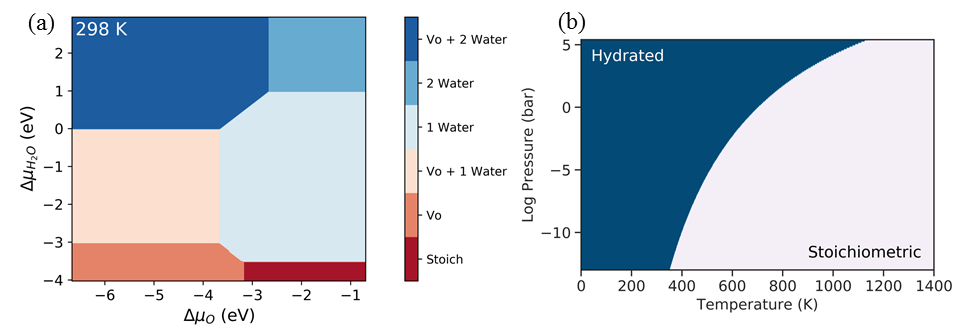
\includegraphics[width=6in]{../Figure_1.png}
    \caption{TODO add Fig}
    \label{Figure 1}
  \end{figure}
  
\section{Acknowledgments}

ARS would like to thank Andrew R. McCluskey for his guidance through this project. This package was written during a PhD funded by AWE and EPSRC (EP/R010366/1). The input
data for the development and testing of this project was generated using ARCHER UK National Supercomputing Service (http://www.archer.ac.uk) via our membership of 
the UK's HEC Materials Chemistry Consortium funded by EPSRC (EP/L000202). 

\bibliography{paper}

\end{document}